% -*- mode: latex; TeX-master: "Vorbis_I_spec"; -*-
%!TEX root = Vorbis_I_spec.tex
% $Id$
\section{Floor type 1 setup and decode} \label{vorbis:spec:floor1}

\subsection{Overview}

Vorbis floor type one uses a piecewise straight-line representation to
encode a spectral envelope curve. The representation plots this curve
mechanically on a linear frequency axis and a logarithmic (dB)
amplitude axis. The integer plotting algorithm used is similar to
Bresenham's algorithm.



\subsection{Floor 1 format}

\subsubsection{model}

Floor type one represents a spectral curve as a series of
line segments.  Synthesis constructs a floor curve using iterative
prediction in a process roughly equivalent to the following simplified
description:

\begin{itemize}
 \item  the first line segment (base case) is a logical line spanning
from x_0,y_0 to x_1,y_1 where in the base case x_0=0 and x_1=[n], the
full range of the spectral floor to be computed.

\item the induction step chooses a point x_new within an existing
logical line segment and produces a y_new value at that point computed
from the existing line's y value at x_new (as plotted by the line) and
a difference value decoded from the bitstream packet.

\item floor computation produces two new line segments, one running from
x_0,y_0 to x_new,y_new and from x_new,y_new to x_1,y_1. This step is
performed logically even if y_new represents no change to the
amplitude value at x_new so that later refinement is additionally
bounded at x_new.

\item the induction step repeats, using a list of x values specified in
the codec setup header at floor 1 initialization time.  Computation
is completed at the end of the x value list.

\end{itemize}


Consider the following example, with values chosen for ease of
understanding rather than representing typical configuration:

For the below example, we assume a floor setup with an [n] of 128.
The list of selected X values in increasing order is
0,16,32,48,64,80,96,112 and 128.  In list order, the values interleave
as 0, 128, 64, 32, 96, 16, 48, 80 and 112.  The corresponding
list-order Y values as decoded from an example packet are 110, 20, -5,
-45, 0, -25, -10, 30 and -10.  We compute the floor in the following
way, beginning with the first line:

\begin{center}
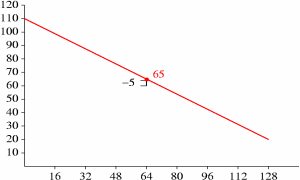
\includegraphics[width=8cm]{floor1-1}
\captionof{figure}{graph of example floor}
\end{center}

We now draw new logical lines to reflect the correction to new_Y, and
iterate for X positions 32 and 96:

\begin{center}
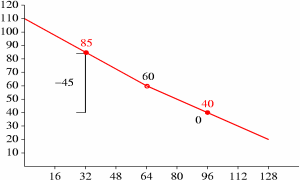
\includegraphics[width=8cm]{floor1-2}
\captionof{figure}{graph of example floor}
\end{center}

Although the new Y value at X position 96 is unchanged, it is still
used later as an endpoint for further refinement.  From here on, the
pattern should be clear; we complete the floor computation as follows:

\begin{center}
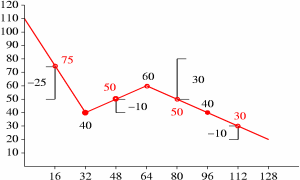
\includegraphics[width=8cm]{floor1-3}
\captionof{figure}{graph of example floor}
\end{center}

\begin{center}
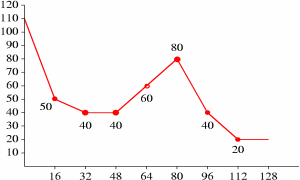
\includegraphics[width=8cm]{floor1-4}
\captionof{figure}{graph of example floor}
\end{center}

A more efficient algorithm with carefully defined integer rounding
behavior is used for actual decode, as described later.  The actual
algorithm splits Y value computation and line plotting into two steps
with modifications to the above algorithm to eliminate noise
accumulation through integer roundoff/truncation.



\subsubsection{header decode}

A list of floor X values is stored in the packet header in interleaved
format (used in list order during packet decode and synthesis).  This
list is split into partitions, and each partition is assigned to a
partition class.  X positions 0 and [n] are implicit and do not belong
to an explicit partition or partition class.

A partition class consists of a representation vector width (the
number of Y values which the partition class encodes at once), a
'subclass' value representing the number of alternate entropy books
the partition class may use in representing Y values, the list of
[subclass] books and a master book used to encode which alternate
books were chosen for representation in a given packet.  The
master/subclass mechanism is meant to be used as a flexible
representation cascade while still using codebooks only in a scalar
context.

\begin{Verbatim}[commandchars=\\\{\}]

  1) [floor1\_partitions] = read 5 bits as unsigned integer
  2) [maximum\_class] = -1
  3) iterate [i] over the range 0 ... [floor1\_partitions]-1 \{

        4) vector [floor1\_partition\_class\_list] element [i] = read 4 bits as unsigned integer

     \}

  5) [maximum\_class] = largest integer scalar value in vector [floor1\_partition\_class\_list]
  6) iterate [i] over the range 0 ... [maximum\_class] \{

        7) vector [floor1\_class\_dimensions] element [i] = read 3 bits as unsigned integer and add 1
	8) vector [floor1\_class\_subclasses] element [i] = read 2 bits as unsigned integer
        9) if ( vector [floor1\_class\_subclasses] element [i] is nonzero ) \{

             10) vector [floor1\_class\_masterbooks] element [i] = read 8 bits as unsigned integer

           \}

       11) iterate [j] over the range 0 ... (2 exponent [floor1\_class\_subclasses] element [i]) - 1 \{

             12) array [floor1\_subclass\_books] element [i],[j] =
                 read 8 bits as unsigned integer and subtract one
           \}
      \}

 13) [floor1\_multiplier] = read 2 bits as unsigned integer and add one
 14) [rangebits] = read 4 bits as unsigned integer
 15) vector [floor1\_X\_list] element [0] = 0
 16) vector [floor1\_X\_list] element [1] = 2 exponent [rangebits];
 17) [floor1\_values] = 2
 18) iterate [i] over the range 0 ... [floor1\_partitions]-1 \{

       19) [current\_class\_number] = vector [floor1\_partition\_class\_list] element [i]
       20) iterate [j] over the range 0 ... ([floor1\_class\_dimensions] element [current\_class\_number])-1 \{
             21) vector [floor1\_X\_list] element ([floor1\_values]) =
                 read [rangebits] bits as unsigned integer
             22) increment [floor1\_values] by one
           \}
     \}

 23) done
\end{Verbatim}

An end-of-packet condition while reading any aspect of a floor 1
configuration during setup renders a stream undecodable.  In addition,
a \varname{[floor1\_class\_masterbooks]} or
\varname{[floor1\_subclass\_books]} scalar element greater than the
highest numbered codebook configured in this stream is an error
condition that renders the stream undecodable.  Vector
[floor1\_x\_list] is limited to a maximum length of 65 elements; a
setup indicating more than 65 total elements (including elements 0 and
1 set prior to the read loop) renders the stream undecodable.  All
vector [floor1\_x\_list] element values must be unique within the
vector; a non-unique value renders the stream undecodable.

\subsubsection{packet decode} \label{vorbis:spec:floor1-decode}

Packet decode begins by checking the \varname{[nonzero]} flag:

\begin{Verbatim}[commandchars=\\\{\}]
  1) [nonzero] = read 1 bit as boolean
\end{Verbatim}

If \varname{[nonzero]} is unset, that indicates this channel contained
no audio energy in this frame.  Decode immediately returns a status
indicating this floor curve (and thus this channel) is unused this
frame.  (A return status of 'unused' is different from decoding a
floor that has all points set to minimum representation amplitude,
which happens to be approximately -140dB).


Assuming \varname{[nonzero]} is set, decode proceeds as follows:

\begin{Verbatim}[commandchars=\\\{\}]
  1) [range] = vector \{ 256, 128, 86, 64 \} element ([floor1\_multiplier]-1)
  2) vector [floor1\_Y] element [0] = read \link{vorbis:spec:ilog}{ilog}([range]-1) bits as unsigned integer
  3) vector [floor1\_Y] element [1] = read \link{vorbis:spec:ilog}{ilog}([range]-1) bits as unsigned integer
  4) [offset] = 2;
  5) iterate [i] over the range 0 ... [floor1\_partitions]-1 \{

       6) [class] = vector [floor1\_partition\_class]  element [i]
       7) [cdim]  = vector [floor1\_class\_dimensions] element [class]
       8) [cbits] = vector [floor1\_class\_subclasses] element [class]
       9) [csub]  = (2 exponent [cbits])-1
      10) [cval]  = 0
      11) if ( [cbits] is greater than zero ) \{

             12) [cval] = read from packet using codebook number
                 (vector [floor1\_class\_masterbooks] element [class]) in scalar context
          \}

      13) iterate [j] over the range 0 ... [cdim]-1 \{

             14) [book] = array [floor1\_subclass\_books] element [class],([cval] bitwise AND [csub])
             15) [cval] = [cval] right shifted [cbits] bits
	     16) if ( [book] is not less than zero ) \{

	           17) vector [floor1\_Y] element ([j]+[offset]) = read from packet using codebook
                       [book] in scalar context

                 \} else [book] is less than zero \{

	           18) vector [floor1\_Y] element ([j]+[offset]) = 0

                 \}
          \}

      19) [offset] = [offset] + [cdim]

     \}

 20) done
\end{Verbatim}

An end-of-packet condition during curve decode should be considered a
nominal occurrence; if end-of-packet is reached during any read
operation above, floor decode is to return 'unused' status as if the
\varname{[nonzero]} flag had been unset at the beginning of decode.


Vector \varname{[floor1\_Y]} contains the values from packet decode
needed for floor 1 synthesis.



\subsubsection{curve computation} \label{vorbis:spec:floor1-synth}

Curve computation is split into two logical steps; the first step
derives final Y amplitude values from the encoded, wrapped difference
values taken from the bitstream.  The second step plots the curve
lines.  Also, although zero-difference values are used in the
iterative prediction to find final Y values, these points are
conditionally skipped during final line computation in step two.
Skipping zero-difference values allows a smoother line fit.

Although some aspects of the below algorithm look like inconsequential
optimizations, implementors are warned to follow the details closely.
Deviation from implementing a strictly equivalent algorithm can result
in serious decoding errors.

{\em Additional note:} Although \varname{[floor1\_final\_Y]} values in
the prediction loop and at the end of step 1 are inherently limited by
the prediction algorithm to [0, \varname{[range]}), it is possible to
  abuse the setup and codebook machinery to produce negative or
  over-range results.  We suggest that decoder implementations guard
  the values in vector \varname{[floor1\_final\_Y]} by clamping each
  element to [0, \varname{[range]}) after step 1.  Variants of this
    suggestion are acceptable as valid floor1 setups cannot produce
    out of range values.

\begin{description}
\item[step 1: amplitude value synthesis]

Unwrap the always-positive-or-zero values read from the packet into
+/- difference values, then apply to line prediction.

\begin{Verbatim}[commandchars=\\\{\}]
  1) [range] = vector \{ 256, 128, 86, 64 \} element ([floor1\_multiplier]-1)
  2) vector [floor1\_step2\_flag] element [0] = set
  3) vector [floor1\_step2\_flag] element [1] = set
  4) vector [floor1\_final\_Y] element [0] = vector [floor1\_Y] element [0]
  5) vector [floor1\_final\_Y] element [1] = vector [floor1\_Y] element [1]
  6) iterate [i] over the range 2 ... [floor1\_values]-1 \{

       7) [low\_neighbor\_offset] = \link{vorbis:spec:low:neighbor}{low\_neighbor}([floor1\_X\_list],[i])
       8) [high\_neighbor\_offset] = \link{vorbis:spec:high:neighbor}{high\_neighbor}([floor1\_X\_list],[i])

       9) [predicted] = \link{vorbis:spec:render:point}{render\_point}( vector [floor1\_X\_list] element [low\_neighbor\_offset],
				      vector [floor1\_final\_Y] element [low\_neighbor\_offset],
                                      vector [floor1\_X\_list] element [high\_neighbor\_offset],
				      vector [floor1\_final\_Y] element [high\_neighbor\_offset],
                                      vector [floor1\_X\_list] element [i] )

      10) [val] = vector [floor1\_Y] element [i]
      11) [highroom] = [range] - [predicted]
      12) [lowroom]  = [predicted]
      13) if ( [highroom] is less than [lowroom] ) \{

            14) [room] = [highroom] * 2

          \} else [highroom] is not less than [lowroom] \{

            15) [room] = [lowroom] * 2

          \}

      16) if ( [val] is nonzero ) \{

            17) vector [floor1\_step2\_flag] element [low\_neighbor\_offset] = set
            18) vector [floor1\_step2\_flag] element [high\_neighbor\_offset] = set
            19) vector [floor1\_step2\_flag] element [i] = set
            20) if ( [val] is greater than or equal to [room] ) \{

                  21) if ( [highroom] is greater than [lowroom] ) \{

                        22) vector [floor1\_final\_Y] element [i] = [val] - [lowroom] + [predicted]

		      \} else [highroom] is not greater than [lowroom] \{

                        23) vector [floor1\_final\_Y] element [i] = [predicted] - [val] + [highroom] - 1

                      \}

                \} else [val] is less than [room] \{

                    24) if ([val] is odd) \{

                        25) vector [floor1\_final\_Y] element [i] =
                            [predicted] - (([val] + 1) divided by  2 using integer division)

                      \} else [val] is even \{

                        26) vector [floor1\_final\_Y] element [i] =
                            [predicted] + ([val] / 2 using integer division)

                      \}

                \}

          \} else [val] is zero \{

            27) vector [floor1\_step2\_flag] element [i] = unset
            28) vector [floor1\_final\_Y] element [i] = [predicted]

          \}

     \}

 29) done

\end{Verbatim}



\item[step 2: curve synthesis]

Curve synthesis generates a return vector \varname{[floor]} of length
\varname{[n]} (where \varname{[n]} is provided by the decode process
calling to floor decode).  Floor 1 curve synthesis makes use of the
\varname{[floor1\_X\_list]}, \varname{[floor1\_final\_Y]} and
\varname{[floor1\_step2\_flag]} vectors, as well as [floor1\_multiplier]
and [floor1\_values] values.

Decode begins by sorting the scalars from vectors
\varname{[floor1\_X\_list]}, \varname{[floor1\_final\_Y]} and
\varname{[floor1\_step2\_flag]} together into new vectors
\varname{[floor1\_X\_list]'}, \varname{[floor1\_final\_Y]'} and
\varname{[floor1\_step2\_flag]'} according to ascending sort order of the
values in \varname{[floor1\_X\_list]}.  That is, sort the values of
\varname{[floor1\_X\_list]} and then apply the same permutation to
elements of the other two vectors so that the X, Y and step2\_flag
values still match.

Then compute the final curve in one pass:

\begin{Verbatim}[commandchars=\\\{\}]
  1) [hx] = 0
  2) [lx] = 0
  3) [ly] = vector [floor1\_final\_Y]' element [0] * [floor1\_multiplier]
  4) iterate [i] over the range 1 ... [floor1\_values]-1 \{

       5) if ( [floor1\_step2\_flag]' element [i] is set ) \{

             6) [hy] = [floor1\_final\_Y]' element [i] * [floor1\_multiplier]
 	     7) [hx] = [floor1\_X\_list]' element [i]
             8) \link{vorbis:spec:render:line}{render\_line}( [lx], [ly], [hx], [hy], [floor] )
             9) [lx] = [hx]
	    10) [ly] = [hy]
          \}
     \}

 11) if ( [hx] is less than [n] ) \{

        12) \link{vorbis:spec:render:line}{render\_line}( [hx], [hy], [n], [hy], [floor] )

     \}

 13) if ( [hx] is greater than [n] ) \{

            14) truncate vector [floor] to [n] elements

     \}

 15) for each scalar in vector [floor], perform a lookup substitution using
     the scalar value from [floor] as an offset into the vector \link{vorbis:spec:floor1:inverse:dB:table}{[floor1\_inverse\_dB\_static\_table]}

 16) done

\end{Verbatim}

\end{description}
